\documentclass[10pt]{article} 
\usepackage{a4} 
\usepackage{makeidx}
\usepackage[danish]{babel} 
\usepackage[utf8]{inputenc}
\usepackage{textcomp}
\usepackage{amsmath}
\usepackage{amssymb}
\usepackage{amsthm}
\usepackage{graphicx} 
\usepackage{verbatim} 
\usepackage{fancyhdr}
\usepackage{listings} 
\usepackage{url}
\frenchspacing
\makeindex
\pagestyle{plain}
\newcommand{\Oh}[0]{ \mathcal{O} }
%\addtolength{\voffset}{-70pt}
%\addtolength{\textheight}{70pt}

%\addtolength{\hoffset}{-40pt}
%\addtolength{\textwidth}{80pt}

\lstset{language=Python}
\title{Grundlæggende datalogi}
\author{RasmusJensen@kommunikationogit.dk}
\date{30/8 2009}

\begin{document}

\maketitle
\tableofcontents

\section{Ugeseddel, uge 36}
Undervisningen starter første gang på torsdag d. 3/9, klokken 8:00, lokale 18.1.59 på KUA.

Forrige torsdag var der introduktion, hvor I fik installeret udviklingsmiljøet JES (Jython Environment for Students), og I kom i gang med at lave nogle små programmer i dette.
I den forbindelse nævnte jeg lidt om:
\begin{itemize}
\item Overblik over JES
\item Kald af funktioner
\item Datatyper: tekst, tal og billeder
\item Variable (navngivning)
\item Grafik i JES.
\item Definition og kald af egne funktioner
\end{itemize}
hvilket vi arbejder videre med i denne uge. 
Derudover kommer vi også til at kigge lidt på dokumentation og kommentarer, samt repræsentation af billeder.


\subsection{Litteratur} 
Bogen er endnu ikke ankommet til bogladen.
Som nødløsning er der nogle hurtige noter herunder.
Læs derudover dele af den indbyggede hjælp i JES, der også indeholder introduktion til programmering: ``Help''-``Getting Started with JES'',  ``Help''-``Programming in Jython'' og ``Help''-``Understanding Pictures in JES''

\subsection{Øvelser d. 3/9}
Bliver udleveret med opdateret ugeseddel, - afhænger delvist af om bogen når at komme i bogladen inden onsdag.

\subsection{Aflevering}
Send en email, senest d. 6/9-2009, med:
\begin{itemize}
\item Et par ord om jer selv, jeres forhold til IT, om I har programmeret før og i så fald hvad, etc. så jeg kan få en bedre fornemmelse af holdet.
\item Et program i JES, der genererer, eller modificerer, et billede. 
Formålet med dette er at I blive fortrolige med repræsentationen af billeder, samt anvendelse og definition af funktioner. 
Tag eventuelt udgangspunkt i eksemplet i noterne, og byg videre på dette.
\end{itemize}

\section{Introduktion til programmering i JES}
\begin{figure}
\begin{center}
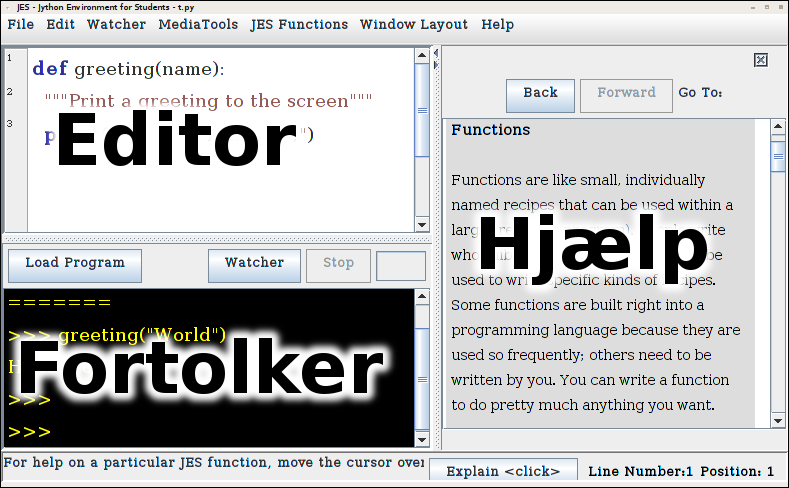
\includegraphics[width=350pt]{JESdesc.png}
\caption{Programmet JES (Jython Environment for Students)}
\label{JES}
\end{center}
\end{figure}

Til at starte med programmere vi i JES (Jython Environment for Students).
Når det kører, ser det omtrent ud som vist på figur~\ref{JES}.
Vinduet er delt op i to-tre dele: en editor hvor man redigere programmer, en fortolker hvor man kan have en interaktiv dialog med python, og et hjælpevindue med dokumentation.

\emph{Editor}en bruges til at skrive og redigere programmerne. Programmer skrevet i python er almindelige tekstfiler, typisk navngivet med \verb|.py| som extension/fileftenavn.
Ændringer i et pythonprogram bliver først indlæst i fortolkeren, når man man trykker på knappen ``Load Program'', og derved også gemmer programmet.

Under editoren er \emph{fortolker}en, som fungere som en interaktiv dialog med python. Kommandoer og udtryk bliver udført direkte her når man skriver dem, og resultatet vises direkte. Her kan der eksperimenteres og laves beregninger.
Fortolkeren angiver med indrykningen \verb|>>>| at her kan der indtastes pythonkode, og svarer uden indrykning. Dette anvendes også i eksempler således at:
\begin{verbatim}
>>> 6*7
42
\end{verbatim}
svarer til at man skriver \verb|6*7| i fortolkeren og trykker enter, hvorefter python svarer ved at skrive \verb|42|.

I menuen ``JES Functions'' findes nogle af de indbyggede funktioner. Når en af disse vælges, bliver den automatisk skrevet editoren eller fortolkervinduet, afhængigt af hvor man står med cursoren. Samtidigt åbnes \emph{hjælp}evinduet med dokmentation af den pågældende funktion.

\subsection{Kald af indbyggede funktioner}
Funktioner indeholder instruktioner til computeren. Eksempelvis hvis man vil have computeren vise et vindue med en hilsen, kan dette gøres ved at udføre/kalde funktionen showInformation:
\begin{verbatim}
>>> showInformation("Hello world")
\end{verbatim}
Dette består af tre dele: 1) navnet på funktionen, {\tt showInformation }, 2) parenteser, der angiver at vi vil udfører funktionen, {\tt ( ) }, samt 3) en tekststreng som parameter til funktionen \verb|"Hello world"|. 
Funktioner kan også retunere værdier:
\begin{verbatim}
>>> requestInteger("Indtast et tal")
2009
\end{verbatim}

\subsection{Datatyper}

JES kan arbejde med forskellige former for datatyper,
eksempelvis tal\footnote{
Bemærk iøvrigt at python skelner mellem heltal og kommatal, hvilket man skal være opmærksom ved eksempelvis division, hvor resultat bliver beskåret til et heltal hvis begge tal er heltal: \\
{ \tt
>>> 100/3\\
33\\
>>> 100/3.0\\
33.333333333333336}\\
Ved beregning med kommatal forkommer også unøjagtigheder på grund af afrunding. Beregningen foregår via binære tal, hvilket medfører at afrundingen ser lidt underlig ud i titalssystemet.
}, tekststrenge, og billeder:
\begin{verbatim}
>>> 5*5+4*4
41
>>> 'Hej ' + 'verden'
'Hej verden'
>>> makeEmptyPicture(100, 100)
Picture, filename None height 100 width 100
\end{verbatim}

Python har en indbygget funktion, \verb|type|, der fortæller typen af data:
\begin{verbatim}
>>> type(123)
<type 'int'>
>>> type('tekststreng')
<type 'str'>
>>> type(showInformation)
<type 'function'>
\end{verbatim}

\subsection{Variable / navngivning}
Tekststreng skrives i anførselstegn, og ord der ikke står i anførselstegn ser python som navne den burde kende:
\begin{verbatim}
>>> pi
3.141592653589793
>>> historie
The error was:historie
Name not found globally.
A local or global name could not be found. You need to define the function or variable before you try to use it in any way.
\end{verbatim}

Variable er navngivne data. Man definere en variabel ved brug af lighedstegn, eksempelvis: \verb|historie = "der var engang..."|, hvorefter \verb|historie| ikke længere vil resultere i en fejl men istedet vil have værdien 'der var engang...'.
Dette er blandt andet praktisk til kunne gemme mellemresultater.

\subsection{Grafik}

\begin{figure}
\begin{center}

\includegraphics[width=350pt]{pixelimage.png}
\end{center}
\caption{Et udsnit af pythonlogoet, forstørret så de enkelte pixels kan ses. Udgaven til højre har indtegnet et gitter så det er endnu mere tydeligt.}
\label{pythonlogoudsnit}
\end{figure}

\begin{figure}
\begin{center}
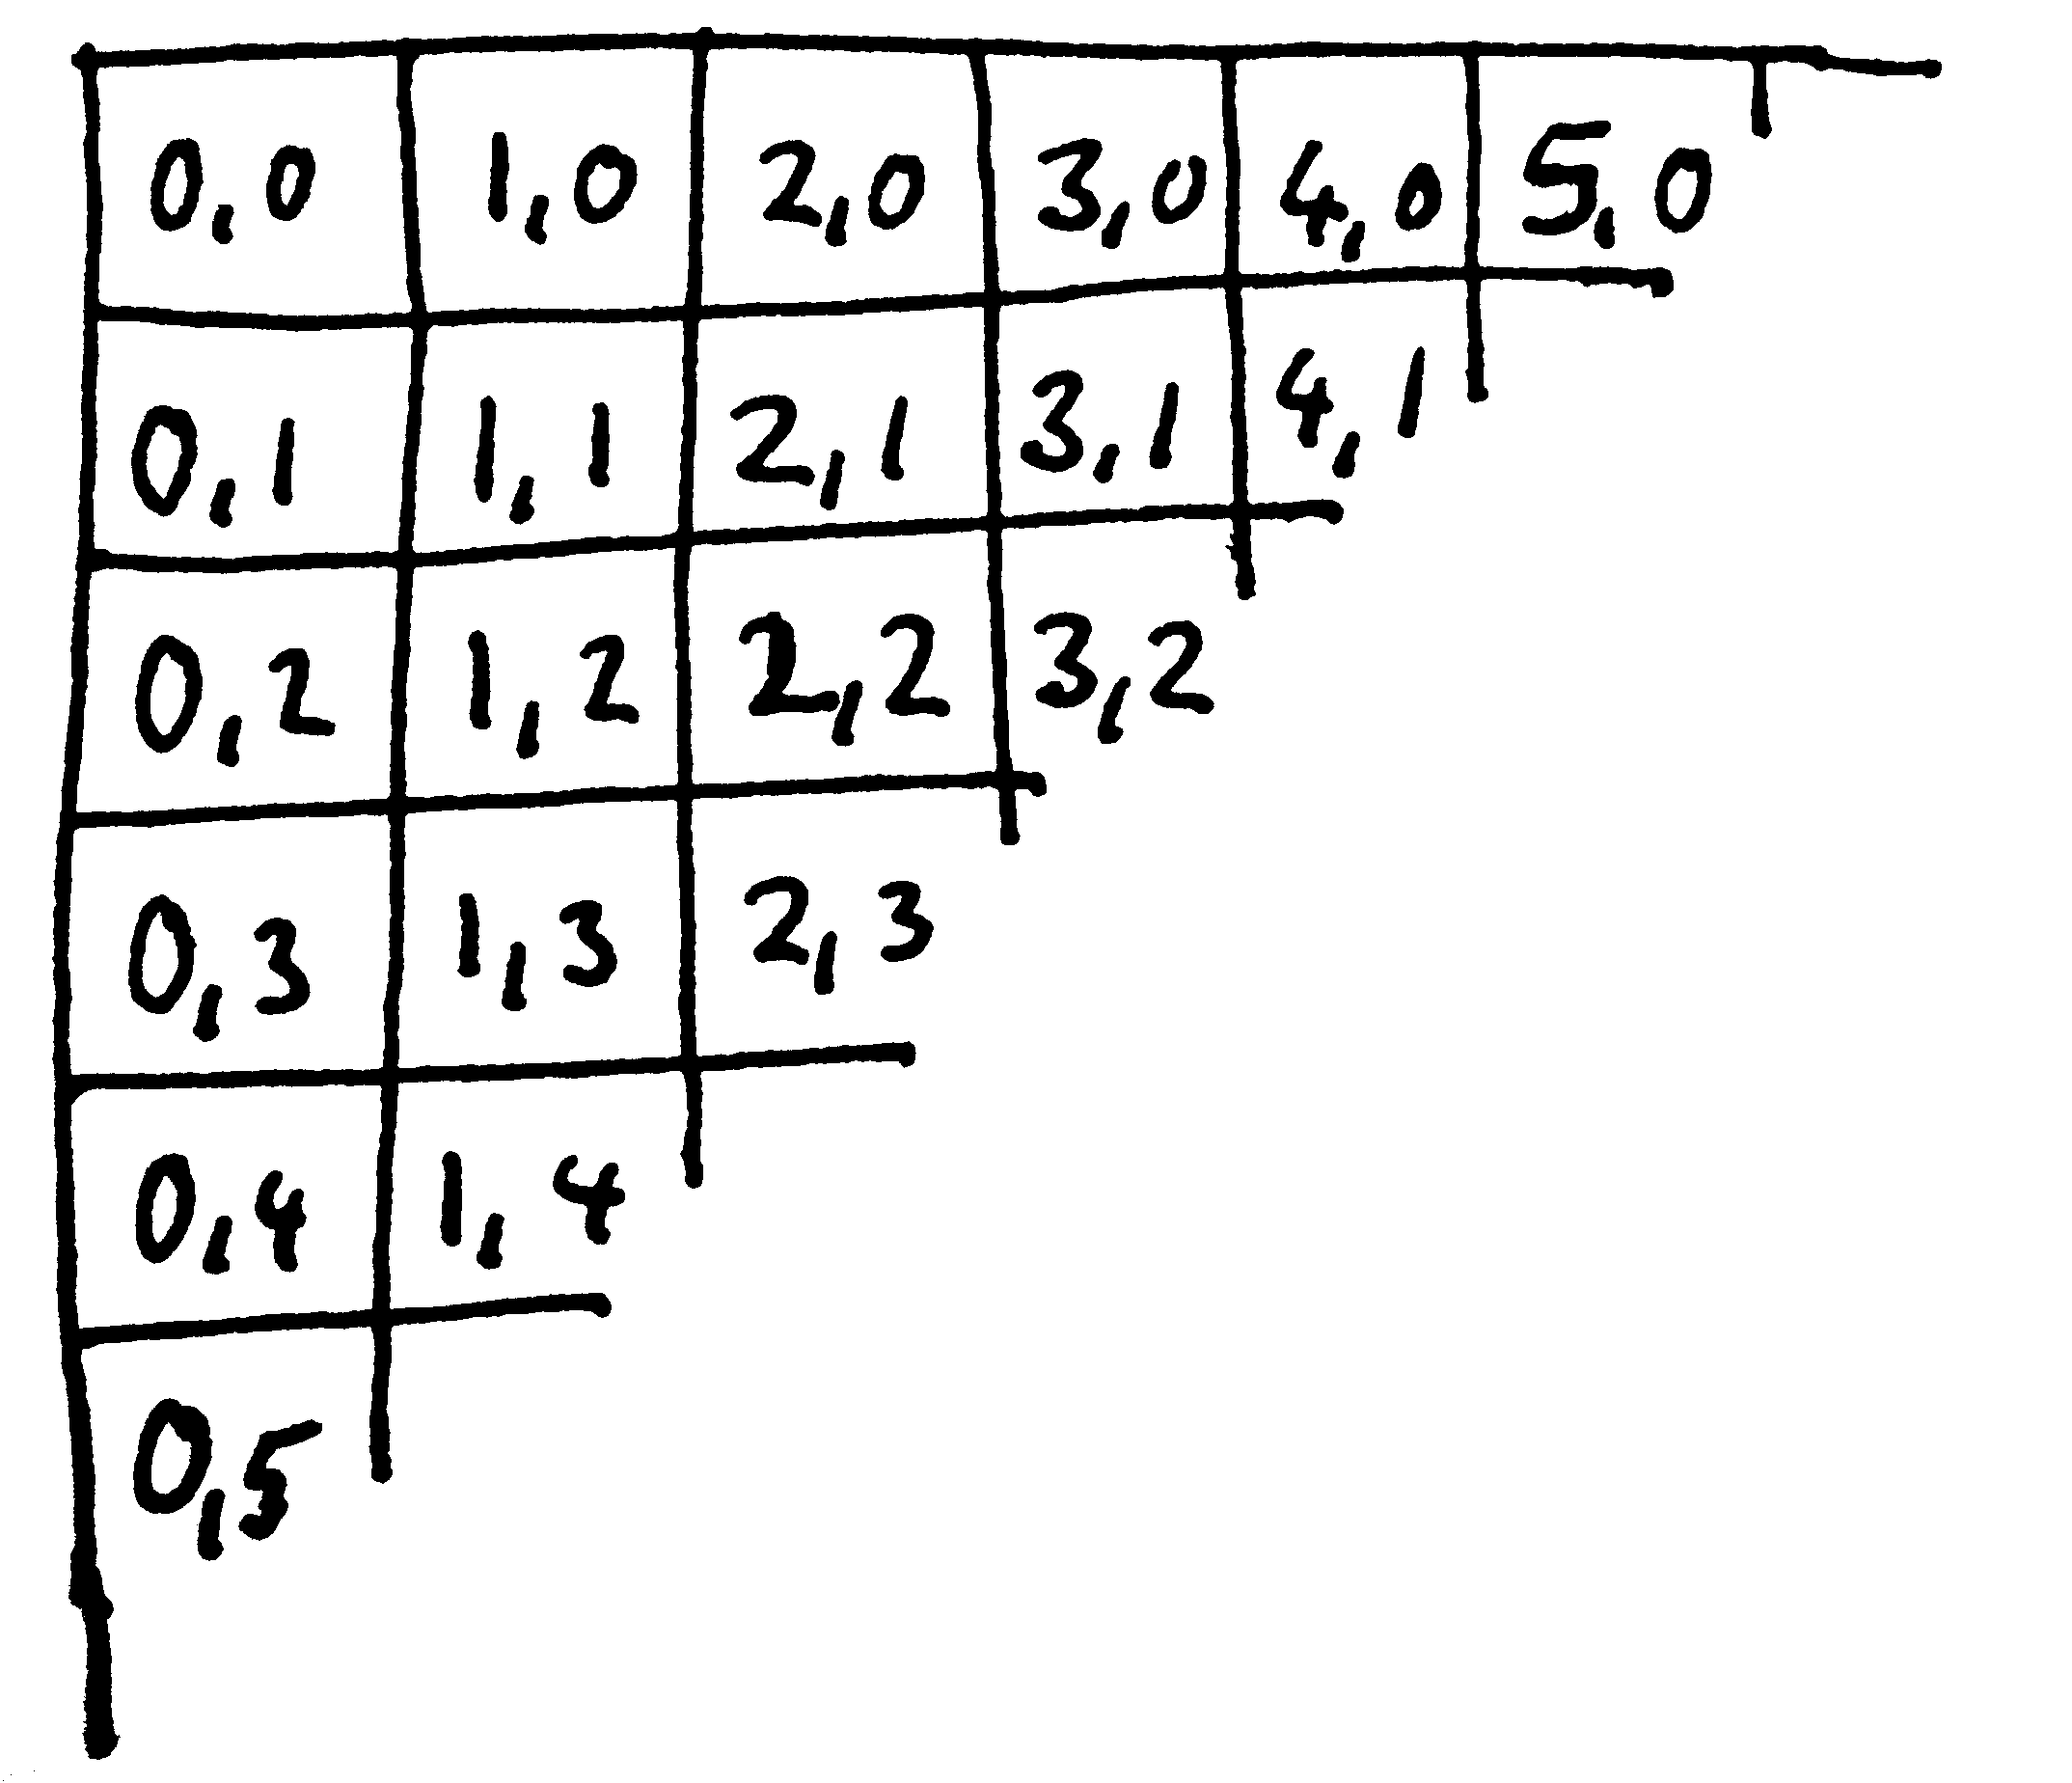
\includegraphics[width=150pt]{pixelpos.png}
\end{center}
\caption{Koordinater for pixels i et billede}
\label{pixelnummer}
\end{figure}

Computeren representere typisk et billede som et gitter af punkter/pixels, hvor hvor hver pixel har en farve. Et eksempel på dette kan ses på figur~\ref{pythonlogoudsnit}.

De enkelte pixels er nummereret med koordinater startende fra øverste venstre hjørne, så den først pixel er $(0,0)$, til højre for denne kommer $(1,0), (2,0), \cdots$, og direkte under den er $(0,1)$. Figur~\ref{pixelnummer} viser denne nummerering.
Derudover har hver enkelt pixel også en farve.

Farver i computeren er repræsenteret ved tre tal der indikerer rød, grøn og blå lysintensitet. 
Når man blander lys-farver er det netop disse tre der er grundfarverne, og disse matcher også hvad øjet biologisk er bygget til at kunne detektere.
I computeren er hver lysintensitet et heltal mellem 0 og 255, og for hver farve er der så tre tal svarende til den røde, grønne og blå lysintensitet. Det vil sige at (255,0,0) er rød, (0,0,0) er sort, (255,255,255) er hvid, (0,255,0) er grøn, (100,100,100) er grå, (0,255,255) er turkis og så fremdeles.

I JES kan en farve laves med funktionen \verb|makeColor|, et tomt billede kan laves med funktionen \verb|makeEmptyPicture|, og et billede kan blive vist med funktionen \verb|show|, så følgende laver et lyserødt billede der er $100\times 100$ pixels:
\begin{verbatim}
>>> lightRed = makeColor(255, 200, 200)
>>> picture = makeEmptyPicture(100, 100, lightRed)
>>> show(picture)
\end{verbatim}

De enkelte pixels i et billede kan findes med funktionen \verb|getPixel|. Når man har fundet en enkelt pixel, kan dennes farve så læses og ændres ved hjælp af \verb|setColor|. Eksempel:
\begin{verbatim}
>>> pixel = getPixel(picture, 10, 10)
>>> setColor(pixel, makeColor(0, 100, 0))
>>> explore(picture)
\end{verbatim}

Bemærk at funktionen getPixel kræver billedet som parameter. Der er også andre funktioner der ændre billedet, eksempelvis ved at tegne på det. Se også dokumentationen i JES i menuen ``Help''-``Understanding Pictures''

\subsection{Kommentarer}

Programmer er ikke kun noget man skriver,
men også noget man læser.
For at gøre det lettere at læse,
kan man vælge fornuftige navne til sine variable,
samt skrive kommentarer.
Kommentarer i programmet bliver ignoreret af computeren,
men kan gøre det lettere for mennesker at
forstå hvad der sker. I python starter en kommentar med \verb|#| hvorefter computeren ignorerer resten af linjen. Eksempel:
\verbatiminput{smiley.py}

\subsection{Definition af funktioner}
Vi har foreløbig kigge på hvorledes man kalder funktioner.
Det er også muligt selv at definere funktioner, 
hvilket eksempelvis kan gøres således:
\begin{verbatim}
def funktionsnavn(parameter1, parameter2):
    printNow("Summen er: " + str(parameter1 + parameter2))
    printNow("Produktet er: " + str(parameter1 * parameter2))
\end{verbatim}
Hvorefter det vil være muligt at kalde funktionen ved eksempelvis at skrive \verb|funktionsnavn(4, 5)|, hvorefter sum og produkt af de to tal bliver skrevet ud.
Bemærk at parametre er lokale variable, hvilket vil sige at i eksemplet bliver \verb|parameter1| sat til at have værdien 4 og \verb|parameter2| sat til 5, hvorefter alt det der står indrykket efter \verb|def| vil blive udført.
Et eksempel på brug af funktioner til at lave lidt grafik med er:
\verbatiminput{eksempel.py}

\begin{comment}
\section{Plan for i dag}
\begin{itemize}
\item Introduktion til kurset Grundlæggende Datalogi
\item Installér JES
\item Leg med Python
\end{itemize}

\section{Installation af JES}
... om programmering, 
-
overblik over programmet
\section{I gang med Python}
\subsection{Kald af funktioner}

\subsection{Regnemaskine og tekst}
\paragraph{Øvelse:} Prøv at bruge fortolkeren som en lommeregner
\subsection{Debugging}
... følsomhed for korrekt syntaks
... eksperimenter i fortolkeren
... ikke danske bogstaver
\subsection{Variable (navngivning)}
\paragraph{Eksempel:} 

\end{comment}


\end{document}

